\begin{figure}[!]
    \centering
    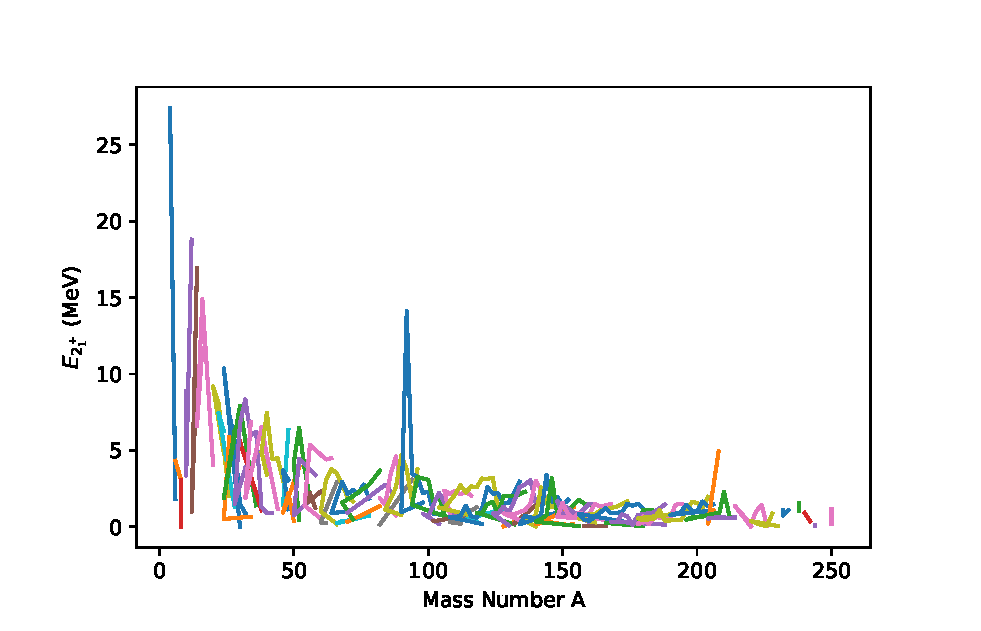
\includegraphics[scale=0.9]{Introduction_Figs/E2vsA.eps}
    \caption{The energy of the first excited $2^+$ state, plotted in isotopic chains by mass, distinguished by color. Areas of high excitation energy, around A$\sim$90,140,210 all correspond to doubly magic areas. The areas around A$\sim$110,170 have much lower excitation energies and correspond to areas of deformation. }
    \label{fig:E2bymass}
\end{figure}